% ============================================================================
%  Results -- % ============================================================================
%  Results -- % ============================================================================
%  Results -- % ============================================================================
%  Results -- \input{sections/results}
%  Numbers come from tables/*.tex and tables/macros.tex, generated by
%  scripts/make_paper_assets.py from the run folders. Re-run it after new runs.
%  Sentences marked \todo{} state a claim that must be checked against the
%  final numbers (keep, reverse or delete).
% ============================================================================
\section{Results}
\label{sec:results}

\subsection{Comparison with the state of the art}
\label{sec:main}
Table~\ref{tab:main} lists the published results on AV-FFIA with their protocols, followed by our models
under the official split. The distilled quaternion model, HyperAVNet-Q (KD), reaches
\resOurAcc\,\% accuracy (macro-F1 \resOurFone\,\%) with \resOurParams\,M parameters and
\resOurGMACs\,GMACs per clip. That is 10.1$\times$ fewer parameters and 13.1$\times$ fewer MACs than
U-FFIA~\cite{cui2024uffia}, and 16.4$\times$ / 51.6$\times$ fewer than the cross-attention model.
\todo{Position against the strongest comparable result: DynaGate-AV reports 96.4--96.5\% on the same
official split rule, and HMMF-Net 96.77\% under 5-fold CV (Table~\ref{tab:protocols}). State whether
HyperAVNet exceeds, matches or trails them; LDMF and HMKD use filtered subsets and are not comparable.}
Fig.~\ref{fig:acc_compute} places all models on an accuracy--compute plane.
Its single-modality heads reach \resOurAccA\,\% (audio) and \resOurAccV\,\% (video), against the
best published single-modality models, Pre-CNN10 (85.9\%) and Pretrained-S3D (89.8\%)~\cite{cui2024uffia}.

\begin{table*}[t]
  \centering
  \caption{Comparison on AV-FFIA. Compute is in GMACs per 2\,s clip; U-FFIA's ``FLOPs'' are MACs.
  Published numbers are quoted with their own protocol and are not directly comparable across
  protocols. $^\dagger$Not verified against the full paper (taken from secondary sources). Our
  rows: official split, mean $\pm$ std over three seeds.}
  \label{tab:main}
  \small
  \resizebox{\textwidth}{!}{\input{tables/main.tex}}
\end{table*}

\begin{figure}[t]
  \centering
  \IfFileExists{figures/acc_vs_compute.pdf}{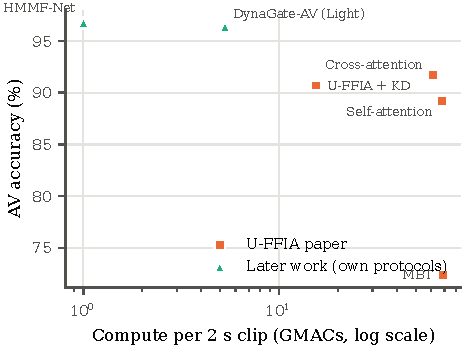
\includegraphics[width=\columnwidth]{figures/acc_vs_compute.pdf}}{\fbox{\parbox{0.9\columnwidth}{\centering run \texttt{scripts/make\_paper\_assets.py}}}}
  \caption{Accuracy versus compute (log scale) on AV-FFIA. Published models are plotted at their
  reported values and protocols; HyperAVNet uses the official split.}
  \label{fig:acc_compute}
\end{figure}

\subsection{Where to fuse: the deep-to-early study}
\label{sec:depth}
Table~\ref{tab:depth} and Fig.~\ref{fig:depth} vary the fusion set $\mathcal{S}$. Late fusion
($\mathcal{S}=\{3\}$) gives \resLateAcc\,\%; progressive fusion from stage~1 gives \resProgAcc\,\%;
the best setting is $\mathcal{S}=\resBestDepth$. Fusion is nearly free in compute: each additional HCF
stage costs about 0.17\,M parameters and under 0.02\,GMACs. Disabling the cross-modal feedback of
Eq.~\eqref{eq:feedback} at $\mathcal{S}=\{1,2,3\}$ gives \resNoFeedbackAcc\,\%.
\todo{Interpret: does accuracy grow as fusion moves earlier, saturate, or peak at mid-level stages
(an inverted U)? Does feedback help, and does the gain concentrate on Weak and Medium? Use the
single-stage rows to locate the most useful depth.}

\begin{table}[t]
  \centering
  \caption{Fusion depth (deep to early) and cross-modal feedback. Mean $\pm$ std, official split.}
  \label{tab:depth}
  \footnotesize
  \setlength{\tabcolsep}{3pt}
  \resizebox{\columnwidth}{!}{\input{tables/ablation_depth.tex}}
\end{table}

\begin{figure}[t]
  \centering
  \IfFileExists{figures/fusion_depth.pdf}{\includegraphics[width=\columnwidth]{figures/fusion_depth.pdf}}{\fbox{\parbox{0.9\columnwidth}{\centering pending runs \texttt{A\_fs*}}}}
  \caption{Accuracy as fusion moves from the last stage to all stages, with and without feedback.}
  \label{fig:depth}
\end{figure}

\subsection{Effect of the hypercomplex algebra}
\label{sec:algebra}
Table~\ref{tab:algebra} and Fig.~\ref{fig:algebra} replace every hypercomplex layer of the network with
algebra $\mathbb{A}_n$. All variants share the architecture and compute and differ only in weight
sharing. The real network ($n=1$, 7.88\,M parameters) reaches \resRealAcc\,\%, the quaternion network
(2.14\,M) \resQuatAcc\,\% and the octonion network (1.24\,M) \resOctAcc\,\%.
\todo{Interpret: if accuracy is maintained or improved down to $n=4$ or $n=8$, the Hamilton
weight sharing acts as a useful structural prior on a dataset of this size; report where accuracy
starts to drop.}

\begin{table}[t]
  \centering
  \caption{Algebra of the whole network. Compute is identical for all $n$.}
  \label{tab:algebra}
  \footnotesize
  \resizebox{\columnwidth}{!}{\input{tables/ablation_algebra.tex}}
\end{table}

\begin{figure}[t]
  \centering
  \IfFileExists{figures/algebra.pdf}{\includegraphics[width=\columnwidth]{figures/algebra.pdf}}{\fbox{\parbox{0.9\columnwidth}{\centering pending runs \texttt{B\_n*}}}}
  \caption{Accuracy against parameter count for real, complex, quaternion, octonion and sedenion networks.}
  \label{fig:algebra}
\end{figure}

\subsection{Fusion operator, regularisers and front-end}
\label{sec:operators}
Table~\ref{tab:ops} compares HCF with a hypercomplex attention bottleneck (MBT) at equal parameters,
and with gated concatenation. HCF with quaternion components gives \resHCFAcc\,\% and MBT
\resMBTAcc\,\%. In~\cite{cui2024uffia}, MBT also trailed cross-attention by a wide margin
(72.4\% vs.\ 91.7\%), which the authors attributed to attending to the modalities one after the other.
\todo{State whether parallel reading plus Hamilton mixing closes this gap, and whether octonion
components (four extra interaction terms, same parameters) help.}
The lower block of Table~\ref{tab:ops} isolates modality dropout, the auxiliary heads and the SimPF
front-end~\cite{liu2023simpf}.

\begin{table}[t]
  \centering
  \caption{Fusion operator (top), regularisers (middle) and audio front-end (bottom).}
  \label{tab:ops}
  \footnotesize
  \setlength{\tabcolsep}{3pt}
  \resizebox{\columnwidth}{!}{\input{tables/ablation_fusion_reg.tex}}
\end{table}

\subsection{Which teacher? Teacher ablation}
\label{sec:teachers}
Table~\ref{tab:teachers} reports each teacher's audio-visual and unimodal accuracy, and the accuracy
of the student distilled from it; $\Delta$ is student minus teacher. Fig.~\ref{fig:teachers} plots
student against teacher accuracy. Distillation from the default teacher (CNN10 + S3D,
\resTeacherAcc\,\%) changes the student's accuracy by \resKDGain\ points over the same student trained
without a teacher (\resNoKDAcc\,\%).
\todo{Interpret: does a stronger teacher yield a stronger student, or does the compact HMKD pair (T10,
about 1\,GMAC) distil as well as the larger teachers? Do the transformer teachers (T6, T8, T9) under-perform
on AV-FFIA, as AST and ViViT did in~\cite{cui2024uffia}?}

\begin{table*}[t]
  \centering
  \caption{Teacher ablation. Teacher params (M) and GMACs include the HCF fusion network. Student:
  HyperAVNet-Q distilled from that teacher. $\Delta$ = student $-$ teacher accuracy.}
  \label{tab:teachers}
  \small
  \resizebox{\textwidth}{!}{\input{tables/teachers.tex}}
\end{table*}

\begin{figure}[t]
  \centering
  \IfFileExists{figures/teacher_student.pdf}{\includegraphics[width=\columnwidth]{figures/teacher_student.pdf}}{\fbox{\parbox{0.9\columnwidth}{\centering pending teacher runs}}}
  \caption{Teacher accuracy against the accuracy of the student distilled from it (dashed: no distillation).}
  \label{fig:teachers}
\end{figure}

\subsection{Robustness to noise and missing modalities}
\label{sec:robustness}
Table~\ref{tab:robust} and Fig.~\ref{fig:robust} follow the robustness protocol of~\cite{cui2024uffia}.
\todo{Compare the degradation at $-10$\,dB with U-FFIA (90.7\%$\to$72.6\%) and cross-attention
(91.7\%$\to$72.7\%), only if the same bubble and pump noise was used; otherwise describe the results
as indicative. Discuss the missing-modality columns: the auxiliary heads and masked training should
keep useful accuracy when one modality is absent.}

\begin{table*}[t]
  \centering
  \caption{Robustness. Audio noise at the given SNR (U-FFIA protocol); Dark: video intensities
  $\times0.25$; Noise: Gaussian video noise, $\sigma^{2}=0.2$; $-$A / $-$V: audio / video absent.
  Published rows from~\cite{cui2024uffia} (bubble and pump noise).}
  \label{tab:robust}
  \small
  \resizebox{\textwidth}{!}{\input{tables/robustness.tex}}
\end{table*}

\begin{figure}[t]
  \centering
  \IfFileExists{figures/robustness_snr.pdf}{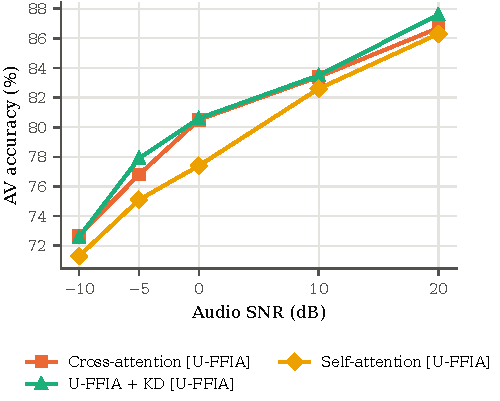
\includegraphics[width=\columnwidth]{figures/robustness_snr.pdf}}{\fbox{\parbox{0.9\columnwidth}{\centering run \texttt{scripts/make\_paper\_assets.py}}}}
  \caption{Audio-visual accuracy as the audio SNR decreases.}
  \label{fig:robust}
\end{figure}

\subsection{Evaluation protocol and data leakage}
\label{sec:protocols}
Table~\ref{tab:protocols} evaluates the same model under the three protocols of Sec.~\ref{sec:setup}:
\resOfficialAcc\,\% on the official split, \resKfoldAcc\,\% under 5-fold CV, and \resGroupedAcc\,\% on
the session-disjoint split.
\todo{If the session-disjoint accuracy is markedly lower, state that clip-level random splits
overestimate generalisation on AV-FFIA, and that published results above 95\% should be read with this
in mind.}

\begin{table}[t]
  \centering
  \caption{One model under three evaluation protocols.}
  \label{tab:protocols}
  \footnotesize
  \resizebox{\columnwidth}{!}{\input{tables/protocols.tex}}
\end{table}

\subsection{Per-class analysis}
\label{sec:perclass}
Table~\ref{tab:perclass} and Fig.~\ref{fig:confusion} give the per-class F1 and the confusion matrix
of HyperAVNet-Q (KD).
\todo{Discuss the dominant confusions, expected between the adjacent intensities Weak and Medium,
and how much the audio stream contributes to separating them.}

\begin{table}[t]
  \centering
  \caption{Per-class F1 of HyperAVNet-Q (KD), official split.}
  \label{tab:perclass}
  \footnotesize
  \input{tables/per_class.tex}
\end{table}

\begin{figure}[t]
  \centering
  \IfFileExists{figures/confusion.pdf}{\includegraphics[width=0.7\columnwidth]{figures/confusion.pdf}}{\fbox{\parbox{0.9\columnwidth}{\centering pending runs}}}
  \caption{Row-normalised confusion matrix (\%) of HyperAVNet-Q (KD), summed over seeds.}
  \label{fig:confusion}
\end{figure}

\subsection{Deployment}
\label{sec:deploy}
Table~\ref{tab:deploy} measures the cost of the two forms of the model on \resDeployDevice{} (batch 1).
In training form, every hypercomplex kernel is assembled from its $n$ blocks at each forward pass.
After reparameterisation (Sec.~\ref{sec:hyper}) the kernels are dense, and latency falls from
\resLatTrain\,ms to \resLatDeploy\,ms. The trade-off is explicit: the hypercomplex form stores and
transmits $n\times$ fewer parameters (2.14\,M), while the deployed dense form holds 7.88\,M parameters
in memory and runs faster. A device can therefore receive the compact model and expand it once at load
time.

\begin{table}[t]
  \centering
  \caption{Training-form versus reparameterised (deployed) model. Stored: parameters kept on disk and
  transmitted; Dense: parameters in memory after reparameterisation.}
  \label{tab:deploy}
  \footnotesize
  \IfFileExists{tables/deploy.tex}{\resizebox{\columnwidth}{!}{\input{tables/deploy.tex}}}{\fbox{run \texttt{profile\_model.py --out}}}
\end{table}

\subsection{Limitations}
\label{sec:limitations}
Hypercomplex layers reduce stored parameters but not arithmetic, so the compute savings come from the
compact backbone design rather than from the algebra. AV-FFIA covers one species and one tank, and
generalisation to farm conditions (turbidity, foam, other species) remains to be shown. Finally, the
discrepancies in the public data release, and the variety of protocols in the literature, limit how
precisely results can be compared across papers.

%  Numbers come from tables/*.tex and tables/macros.tex, generated by
%  scripts/make_paper_assets.py from the run folders. Re-run it after new runs.
%  Sentences marked \todo{} state a claim that must be checked against the
%  final numbers (keep, reverse or delete).
% ============================================================================
\section{Results}
\label{sec:results}

\subsection{Comparison with the state of the art}
\label{sec:main}
Table~\ref{tab:main} lists the published results on AV-FFIA with their protocols, followed by our models
under the official split. The distilled quaternion model, HyperAVNet-Q (KD), reaches
\resOurAcc\,\% accuracy (macro-F1 \resOurFone\,\%) with \resOurParams\,M parameters and
\resOurGMACs\,GMACs per clip. That is 10.1$\times$ fewer parameters and 13.1$\times$ fewer MACs than
U-FFIA~\cite{cui2024uffia}, and 16.4$\times$ / 51.6$\times$ fewer than the cross-attention model.
\todo{Position against the strongest comparable result: DynaGate-AV reports 96.4--96.5\% on the same
official split rule, and HMMF-Net 96.77\% under 5-fold CV (Table~\ref{tab:protocols}). State whether
HyperAVNet exceeds, matches or trails them; LDMF and HMKD use filtered subsets and are not comparable.}
Fig.~\ref{fig:acc_compute} places all models on an accuracy--compute plane.
Its single-modality heads reach \resOurAccA\,\% (audio) and \resOurAccV\,\% (video), against the
best published single-modality models, Pre-CNN10 (85.9\%) and Pretrained-S3D (89.8\%)~\cite{cui2024uffia}.

\begin{table*}[t]
  \centering
  \caption{Comparison on AV-FFIA. Compute is in GMACs per 2\,s clip; U-FFIA's ``FLOPs'' are MACs.
  Published numbers are quoted with their own protocol and are not directly comparable across
  protocols. $^\dagger$Not verified against the full paper (taken from secondary sources). Our
  rows: official split, mean $\pm$ std over three seeds.}
  \label{tab:main}
  \small
  \resizebox{\textwidth}{!}{\begin{tabular}{llrrrrl}
\toprule
Method & Mod. & Params (M) & GMACs & Acc. (\%) & F1 (\%) & Protocol \\
\midrule
Pre-CNN10~\cite{cui2024uffia} & A & 5.00 & 3.347 & 85.9 & -- & paper split \\
Pretrained-S3D~\cite{cui2024uffia} & V & 7.90 & 22.826 & 89.8 & -- & paper split \\
Self-attention~\cite{cui2024uffia} & AV & 47.70 & 68.404 & 89.2 & -- & paper split \\
MBT~\cite{cui2024uffia} & AV & 47.69 & 68.690 & 72.4 & -- & paper split \\
Cross-attention~\cite{cui2024uffia} & AV & 35.08 & 60.933 & 91.7 & -- & paper split \\
U-FFIA + KD~\cite{cui2024uffia} & AV & 21.63 & 15.488 & 90.7 & -- & paper split \\
\midrule
ACAF-Net~\cite{acafnet2025}$^\dagger$ & AV & -- & -- & 95.4 & -- & random split \\
DynaGate-AV (Light)~\cite{dynagate2026} & AV & -- & 5.290 & 96.4 & -- & official split, 19,963 clips \\
HMMF-Net~\cite{hmmfnet2026}$^\dagger$ & AV & 3.99 & 1.002 & 96.8 & 96.9 & 5-fold CV \\
HMKD~\cite{hmkd2026}$^\dagger$ & AV & -- & -- & 97.5 & -- & 26,843-pair holdout \\
LDMF~\cite{ldmf2026}$^\dagger$ & AV & 7.10 & -- & 98.2 & -- & filtered subset \\
\midrule
Real late-concat baseline (ours, re-run) & AV & -- & -- & -- & -- & official split \\
Teacher: CNN10 + S3D + HCF & AV & -- & -- & -- & -- & official split \\
Teacher: EfficientAT + MoViNet-A0 + HCF & AV & -- & -- & -- & -- & official split \\
HyperAVNet-Q (no KD) & AV & -- & -- & -- & -- & official split \\
\textbf{HyperAVNet-Q (KD)} & AV & -- & -- & -- & -- & official split \\
HyperAVNet-P (pretrained, no KD) & AV & -- & -- & -- & -- & official split \\
HyperAVNet-P (pretrained, KD) & AV & -- & -- & -- & -- & official split \\
HyperAVNet-O (KD) & AV & -- & -- & -- & -- & official split \\
\bottomrule
\end{tabular}
}
\end{table*}

\begin{figure}[t]
  \centering
  \IfFileExists{figures/acc_vs_compute.pdf}{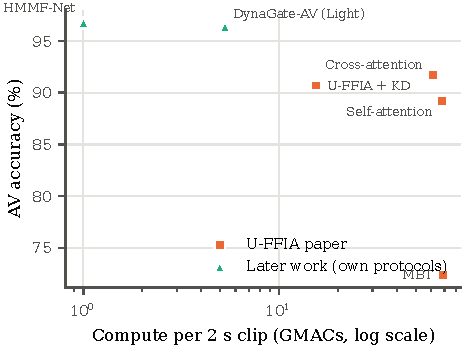
\includegraphics[width=\columnwidth]{figures/acc_vs_compute.pdf}}{\fbox{\parbox{0.9\columnwidth}{\centering run \texttt{scripts/make\_paper\_assets.py}}}}
  \caption{Accuracy versus compute (log scale) on AV-FFIA. Published models are plotted at their
  reported values and protocols; HyperAVNet uses the official split.}
  \label{fig:acc_compute}
\end{figure}

\subsection{Where to fuse: the deep-to-early study}
\label{sec:depth}
Table~\ref{tab:depth} and Fig.~\ref{fig:depth} vary the fusion set $\mathcal{S}$. Late fusion
($\mathcal{S}=\{3\}$) gives \resLateAcc\,\%; progressive fusion from stage~1 gives \resProgAcc\,\%;
the best setting is $\mathcal{S}=\resBestDepth$. Fusion is nearly free in compute: each additional HCF
stage costs about 0.17\,M parameters and under 0.02\,GMACs. Disabling the cross-modal feedback of
Eq.~\eqref{eq:feedback} at $\mathcal{S}=\{1,2,3\}$ gives \resNoFeedbackAcc\,\%.
\todo{Interpret: does accuracy grow as fusion moves earlier, saturate, or peak at mid-level stages
(an inverted U)? Does feedback help, and does the gain concentrate on Weak and Medium? Use the
single-stage rows to locate the most useful depth.}

\begin{table}[t]
  \centering
  \caption{Fusion depth (deep to early) and cross-modal feedback. Mean $\pm$ std, official split.}
  \label{tab:depth}
  \footnotesize
  \setlength{\tabcolsep}{3pt}
  \resizebox{\columnwidth}{!}{\begin{tabular}{lrrrrrr}
\toprule
Fusion stages $\mathcal{S}$ & Params (M) & GMACs & Acc. & F1 & A-only & V-only \\
\midrule
$\{3\}$ (late) & -- & -- & -- & -- & -- & -- \\
$\{2,3\}$ & -- & -- & -- & -- & -- & -- \\
$\{1,2,3\}$ & -- & -- & -- & -- & -- & -- \\
$\{0,1,2,3\}$ & -- & -- & -- & -- & -- & -- \\
\midrule
$\{0\}$ & -- & -- & -- & -- & -- & -- \\
$\{1\}$ & -- & -- & -- & -- & -- & -- \\
$\{2\}$ & -- & -- & -- & -- & -- & -- \\
\midrule
$\{1,2,3\}$ w/o feedback & -- & -- & -- & -- & -- & -- \\
\bottomrule
\end{tabular}
}
\end{table}

\begin{figure}[t]
  \centering
  \IfFileExists{figures/fusion_depth.pdf}{\includegraphics[width=\columnwidth]{figures/fusion_depth.pdf}}{\fbox{\parbox{0.9\columnwidth}{\centering pending runs \texttt{A\_fs*}}}}
  \caption{Accuracy as fusion moves from the last stage to all stages, with and without feedback.}
  \label{fig:depth}
\end{figure}

\subsection{Effect of the hypercomplex algebra}
\label{sec:algebra}
Table~\ref{tab:algebra} and Fig.~\ref{fig:algebra} replace every hypercomplex layer of the network with
algebra $\mathbb{A}_n$. All variants share the architecture and compute and differ only in weight
sharing. The real network ($n=1$, 7.88\,M parameters) reaches \resRealAcc\,\%, the quaternion network
(2.14\,M) \resQuatAcc\,\% and the octonion network (1.24\,M) \resOctAcc\,\%.
\todo{Interpret: if accuracy is maintained or improved down to $n=4$ or $n=8$, the Hamilton
weight sharing acts as a useful structural prior on a dataset of this size; report where accuracy
starts to drop.}

\begin{table}[t]
  \centering
  \caption{Algebra of the whole network. Compute is identical for all $n$.}
  \label{tab:algebra}
  \footnotesize
  \resizebox{\columnwidth}{!}{\begin{tabular}{lrrrr}
\toprule
Algebra & Params (M) & GMACs & Acc. & F1 \\
\midrule
Real ($n{=}1$) & -- & -- & -- & -- \\
Complex ($n{=}2$) & -- & -- & -- & -- \\
Quaternion ($n{=}4$) & -- & -- & -- & -- \\
Octonion ($n{=}8$) & -- & -- & -- & -- \\
Sedenion ($n{=}16$) & -- & -- & -- & -- \\
\bottomrule
\end{tabular}
}
\end{table}

\begin{figure}[t]
  \centering
  \IfFileExists{figures/algebra.pdf}{\includegraphics[width=\columnwidth]{figures/algebra.pdf}}{\fbox{\parbox{0.9\columnwidth}{\centering pending runs \texttt{B\_n*}}}}
  \caption{Accuracy against parameter count for real, complex, quaternion, octonion and sedenion networks.}
  \label{fig:algebra}
\end{figure}

\subsection{Fusion operator, regularisers and front-end}
\label{sec:operators}
Table~\ref{tab:ops} compares HCF with a hypercomplex attention bottleneck (MBT) at equal parameters,
and with gated concatenation. HCF with quaternion components gives \resHCFAcc\,\% and MBT
\resMBTAcc\,\%. In~\cite{cui2024uffia}, MBT also trailed cross-attention by a wide margin
(72.4\% vs.\ 91.7\%), which the authors attributed to attending to the modalities one after the other.
\todo{State whether parallel reading plus Hamilton mixing closes this gap, and whether octonion
components (four extra interaction terms, same parameters) help.}
The lower block of Table~\ref{tab:ops} isolates modality dropout, the auxiliary heads and the SimPF
front-end~\cite{liu2023simpf}.

\begin{table}[t]
  \centering
  \caption{Fusion operator (top), regularisers (middle) and audio front-end (bottom).}
  \label{tab:ops}
  \footnotesize
  \setlength{\tabcolsep}{3pt}
  \resizebox{\columnwidth}{!}{\begin{tabular}{lrrrrr}
\toprule
Variant & Params (M) & Acc. & F1 & A-only & V-only \\
\midrule
HCF, complex components & -- & -- & -- & -- & -- \\
HCF, quaternion components & -- & -- & -- & -- & -- \\
HCF, octonion components & -- & -- & -- & -- & -- \\
Hypercomplex MBT & -- & -- & -- & -- & -- \\
Gated concatenation & -- & -- & -- & -- & -- \\
\midrule
w/o modality dropout ($p{=}0$) & -- & -- & -- & -- & -- \\
modality dropout $p{=}0.25$ & -- & -- & -- & -- & -- \\
w/o auxiliary heads & -- & -- & -- & -- & -- \\
\midrule
SimPF front-end ($k{=}0.5$) & -- & -- & -- & -- & -- \\
\bottomrule
\end{tabular}
}
\end{table}

\subsection{Which teacher? Teacher ablation}
\label{sec:teachers}
Table~\ref{tab:teachers} reports each teacher's audio-visual and unimodal accuracy, and the accuracy
of the student distilled from it; $\Delta$ is student minus teacher. Fig.~\ref{fig:teachers} plots
student against teacher accuracy. Distillation from the default teacher (CNN10 + S3D,
\resTeacherAcc\,\%) changes the student's accuracy by \resKDGain\ points over the same student trained
without a teacher (\resNoKDAcc\,\%).
\todo{Interpret: does a stronger teacher yield a stronger student, or does the compact HMKD pair (T10,
about 1\,GMAC) distil as well as the larger teachers? Do the transformer teachers (T6, T8, T9) under-perform
on AV-FFIA, as AST and ViViT did in~\cite{cui2024uffia}?}

\begin{table*}[t]
  \centering
  \caption{Teacher ablation. Teacher params (M) and GMACs include the HCF fusion network. Student:
  HyperAVNet-Q distilled from that teacher. $\Delta$ = student $-$ teacher accuracy.}
  \label{tab:teachers}
  \small
  \resizebox{\textwidth}{!}{\begin{tabular}{llrrrrrrr}
\toprule
ID & Audio / video teacher & Params & GMACs & Teacher AV & A-only & V-only & Student & $\Delta$ \\
\midrule
T1 & CNN10 / S3D & -- & -- & -- & -- & -- & -- & -- \\
T2 & CNN14 / S3D & -- & -- & -- & -- & -- & -- & -- \\
T3 & CNN10 / R(2+1)D-18 & -- & -- & -- & -- & -- & -- & -- \\
T4 & CNN10 / ConvNeXt-T (frames) & -- & -- & -- & -- & -- & -- & -- \\
T5 & EffNet-B0 (mel) / S3D & -- & -- & -- & -- & -- & -- & -- \\
T6 & AST / VideoMAE-B & -- & -- & -- & -- & -- & -- & -- \\
T7 & CNN10 / X3D-M & -- & -- & -- & -- & -- & -- & -- \\
T8 & AST / S3D & -- & -- & -- & -- & -- & -- & -- \\
T9 & CNN10 / VideoMAE-B & -- & -- & -- & -- & -- & -- & -- \\
T10 & EfficientAT / MoViNet-A0 & -- & -- & -- & -- & -- & -- & -- \\
\midrule
-- & no teacher (no KD) & -- & -- & -- & -- & -- & -- & -- \\
\bottomrule
\end{tabular}
}
\end{table*}

\begin{figure}[t]
  \centering
  \IfFileExists{figures/teacher_student.pdf}{\includegraphics[width=\columnwidth]{figures/teacher_student.pdf}}{\fbox{\parbox{0.9\columnwidth}{\centering pending teacher runs}}}
  \caption{Teacher accuracy against the accuracy of the student distilled from it (dashed: no distillation).}
  \label{fig:teachers}
\end{figure}

\subsection{Robustness to noise and missing modalities}
\label{sec:robustness}
Table~\ref{tab:robust} and Fig.~\ref{fig:robust} follow the robustness protocol of~\cite{cui2024uffia}.
\todo{Compare the degradation at $-10$\,dB with U-FFIA (90.7\%$\to$72.6\%) and cross-attention
(91.7\%$\to$72.7\%), only if the same bubble and pump noise was used; otherwise describe the results
as indicative. Discuss the missing-modality columns: the auxiliary heads and masked training should
keep useful accuracy when one modality is absent.}

\begin{table*}[t]
  \centering
  \caption{Robustness. Audio noise at the given SNR (U-FFIA protocol); Dark: video intensities
  $\times0.25$; Noise: Gaussian video noise, $\sigma^{2}=0.2$; $-$A / $-$V: audio / video absent.
  Published rows from~\cite{cui2024uffia} (bubble and pump noise).}
  \label{tab:robust}
  \small
  \resizebox{\textwidth}{!}{\begin{tabular}{lrrrrrrrrrr}
\toprule
Method & Clean & -10\,dB & -5\,dB & +0\,dB & +10\,dB & +20\,dB & Dark & Noise & $-$A & $-$V \\
\midrule
Cross-attention~\cite{cui2024uffia} & 91.7 & 72.7 & 76.8 & 80.5 & 83.4 & 86.7 & -- & -- & -- & -- \\
U-FFIA + KD~\cite{cui2024uffia} & 90.7 & 72.6 & 77.9 & 80.6 & 83.5 & 87.6 & -- & -- & -- & -- \\
Self-attention~\cite{cui2024uffia} & 89.2 & 71.3 & 75.1 & 77.4 & 82.6 & 86.3 & -- & -- & -- & -- \\
\midrule
Teacher (CNN10 + S3D) & -- & -- & -- & -- & -- & -- & -- & -- & -- & -- \\
\textbf{HyperAVNet-Q (KD)} & -- & -- & -- & -- & -- & -- & -- & -- & -- & -- \\
\bottomrule
\end{tabular}
}
\end{table*}

\begin{figure}[t]
  \centering
  \IfFileExists{figures/robustness_snr.pdf}{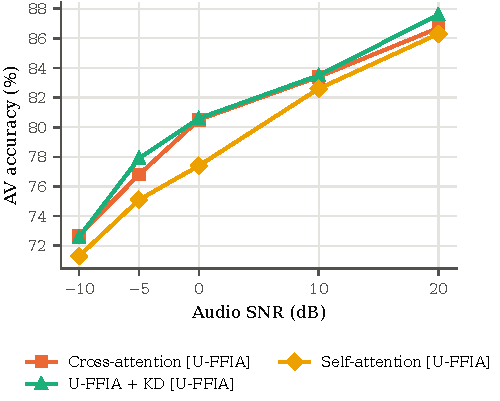
\includegraphics[width=\columnwidth]{figures/robustness_snr.pdf}}{\fbox{\parbox{0.9\columnwidth}{\centering run \texttt{scripts/make\_paper\_assets.py}}}}
  \caption{Audio-visual accuracy as the audio SNR decreases.}
  \label{fig:robust}
\end{figure}

\subsection{Evaluation protocol and data leakage}
\label{sec:protocols}
Table~\ref{tab:protocols} evaluates the same model under the three protocols of Sec.~\ref{sec:setup}:
\resOfficialAcc\,\% on the official split, \resKfoldAcc\,\% under 5-fold CV, and \resGroupedAcc\,\% on
the session-disjoint split.
\todo{If the session-disjoint accuracy is markedly lower, state that clip-level random splits
overestimate generalisation on AV-FFIA, and that published results above 95\% should be read with this
in mind.}

\begin{table}[t]
  \centering
  \caption{One model under three evaluation protocols.}
  \label{tab:protocols}
  \footnotesize
  \resizebox{\columnwidth}{!}{\begin{tabular}{lrrr}
\toprule
Evaluation protocol & Runs & Acc. & F1 \\
\midrule
Official code split (700/700 per class) & -- & -- & -- \\
5-fold stratified CV & -- & -- & -- \\
Session-disjoint (whole recording dates) & -- & -- & -- \\
\bottomrule
\end{tabular}
}
\end{table}

\subsection{Per-class analysis}
\label{sec:perclass}
Table~\ref{tab:perclass} and Fig.~\ref{fig:confusion} give the per-class F1 and the confusion matrix
of HyperAVNet-Q (KD).
\todo{Discuss the dominant confusions, expected between the adjacent intensities Weak and Medium,
and how much the audio stream contributes to separating them.}

\begin{table}[t]
  \centering
  \caption{Per-class F1 of HyperAVNet-Q (KD), official split.}
  \label{tab:perclass}
  \footnotesize
  \begin{tabular}{lr}
\toprule
Class & F1 (\%) \\
\midrule
None & -- \\
Strong & -- \\
Medium & -- \\
Weak & -- \\
\bottomrule
\end{tabular}

\end{table}

\begin{figure}[t]
  \centering
  \IfFileExists{figures/confusion.pdf}{\includegraphics[width=0.7\columnwidth]{figures/confusion.pdf}}{\fbox{\parbox{0.9\columnwidth}{\centering pending runs}}}
  \caption{Row-normalised confusion matrix (\%) of HyperAVNet-Q (KD), summed over seeds.}
  \label{fig:confusion}
\end{figure}

\subsection{Deployment}
\label{sec:deploy}
Table~\ref{tab:deploy} measures the cost of the two forms of the model on \resDeployDevice{} (batch 1).
In training form, every hypercomplex kernel is assembled from its $n$ blocks at each forward pass.
After reparameterisation (Sec.~\ref{sec:hyper}) the kernels are dense, and latency falls from
\resLatTrain\,ms to \resLatDeploy\,ms. The trade-off is explicit: the hypercomplex form stores and
transmits $n\times$ fewer parameters (2.14\,M), while the deployed dense form holds 7.88\,M parameters
in memory and runs faster. A device can therefore receive the compact model and expand it once at load
time.

\begin{table}[t]
  \centering
  \caption{Training-form versus reparameterised (deployed) model. Stored: parameters kept on disk and
  transmitted; Dense: parameters in memory after reparameterisation.}
  \label{tab:deploy}
  \footnotesize
  \IfFileExists{tables/deploy.tex}{\resizebox{\columnwidth}{!}{\begin{tabular}{lrrrrrr}
\toprule
Model & Stored (M) & Dense (M) & GMACs & Train-form (ms) & Deployed (ms) & Speed-up \\
\midrule
-- & -- & -- & -- & -- & -- & -- \\
\bottomrule
\end{tabular}
}}{\fbox{run \texttt{profile\_model.py --out}}}
\end{table}

\subsection{Limitations}
\label{sec:limitations}
Hypercomplex layers reduce stored parameters but not arithmetic, so the compute savings come from the
compact backbone design rather than from the algebra. AV-FFIA covers one species and one tank, and
generalisation to farm conditions (turbidity, foam, other species) remains to be shown. Finally, the
discrepancies in the public data release, and the variety of protocols in the literature, limit how
precisely results can be compared across papers.

%  Numbers come from tables/*.tex and tables/macros.tex, generated by
%  scripts/make_paper_assets.py from the run folders. Re-run it after new runs.
%  Sentences marked \todo{} state a claim that must be checked against the
%  final numbers (keep, reverse or delete).
% ============================================================================
\section{Results}
\label{sec:results}

\subsection{Comparison with the state of the art}
\label{sec:main}
Table~\ref{tab:main} lists the published results on AV-FFIA with their protocols, followed by our models
under the official split. The distilled quaternion model, HyperAVNet-Q (KD), reaches
\resOurAcc\,\% accuracy (macro-F1 \resOurFone\,\%) with \resOurParams\,M parameters and
\resOurGMACs\,GMACs per clip. That is 10.1$\times$ fewer parameters and 13.1$\times$ fewer MACs than
U-FFIA~\cite{cui2024uffia}, and 16.4$\times$ / 51.6$\times$ fewer than the cross-attention model.
\todo{Position against the strongest comparable result: DynaGate-AV reports 96.4--96.5\% on the same
official split rule, and HMMF-Net 96.77\% under 5-fold CV (Table~\ref{tab:protocols}). State whether
HyperAVNet exceeds, matches or trails them; LDMF and HMKD use filtered subsets and are not comparable.}
Fig.~\ref{fig:acc_compute} places all models on an accuracy--compute plane.
Its single-modality heads reach \resOurAccA\,\% (audio) and \resOurAccV\,\% (video), against the
best published single-modality models, Pre-CNN10 (85.9\%) and Pretrained-S3D (89.8\%)~\cite{cui2024uffia}.

\begin{table*}[t]
  \centering
  \caption{Comparison on AV-FFIA. Compute is in GMACs per 2\,s clip; U-FFIA's ``FLOPs'' are MACs.
  Published numbers are quoted with their own protocol and are not directly comparable across
  protocols. $^\dagger$Not verified against the full paper (taken from secondary sources). Our
  rows: official split, mean $\pm$ std over three seeds.}
  \label{tab:main}
  \small
  \resizebox{\textwidth}{!}{\begin{tabular}{llrrrrl}
\toprule
Method & Mod. & Params (M) & GMACs & Acc. (\%) & F1 (\%) & Protocol \\
\midrule
Pre-CNN10~\cite{cui2024uffia} & A & 5.00 & 3.347 & 85.9 & -- & paper split \\
Pretrained-S3D~\cite{cui2024uffia} & V & 7.90 & 22.826 & 89.8 & -- & paper split \\
Self-attention~\cite{cui2024uffia} & AV & 47.70 & 68.404 & 89.2 & -- & paper split \\
MBT~\cite{cui2024uffia} & AV & 47.69 & 68.690 & 72.4 & -- & paper split \\
Cross-attention~\cite{cui2024uffia} & AV & 35.08 & 60.933 & 91.7 & -- & paper split \\
U-FFIA + KD~\cite{cui2024uffia} & AV & 21.63 & 15.488 & 90.7 & -- & paper split \\
\midrule
ACAF-Net~\cite{acafnet2025}$^\dagger$ & AV & -- & -- & 95.4 & -- & random split \\
DynaGate-AV (Light)~\cite{dynagate2026} & AV & -- & 5.290 & 96.4 & -- & official split, 19,963 clips \\
HMMF-Net~\cite{hmmfnet2026}$^\dagger$ & AV & 3.99 & 1.002 & 96.8 & 96.9 & 5-fold CV \\
HMKD~\cite{hmkd2026}$^\dagger$ & AV & -- & -- & 97.5 & -- & 26,843-pair holdout \\
LDMF~\cite{ldmf2026}$^\dagger$ & AV & 7.10 & -- & 98.2 & -- & filtered subset \\
\midrule
Real late-concat baseline (ours, re-run) & AV & -- & -- & -- & -- & official split \\
Teacher: CNN10 + S3D + HCF & AV & -- & -- & -- & -- & official split \\
Teacher: EfficientAT + MoViNet-A0 + HCF & AV & -- & -- & -- & -- & official split \\
HyperAVNet-Q (no KD) & AV & -- & -- & -- & -- & official split \\
\textbf{HyperAVNet-Q (KD)} & AV & -- & -- & -- & -- & official split \\
HyperAVNet-P (pretrained, no KD) & AV & -- & -- & -- & -- & official split \\
HyperAVNet-P (pretrained, KD) & AV & -- & -- & -- & -- & official split \\
HyperAVNet-O (KD) & AV & -- & -- & -- & -- & official split \\
\bottomrule
\end{tabular}
}
\end{table*}

\begin{figure}[t]
  \centering
  \IfFileExists{figures/acc_vs_compute.pdf}{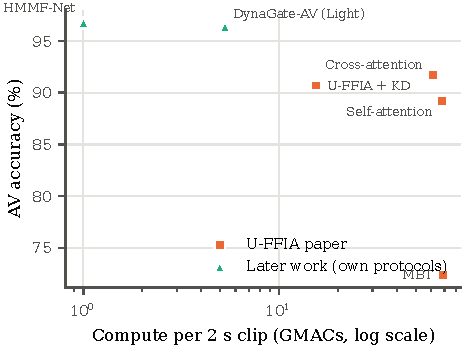
\includegraphics[width=\columnwidth]{figures/acc_vs_compute.pdf}}{\fbox{\parbox{0.9\columnwidth}{\centering run \texttt{scripts/make\_paper\_assets.py}}}}
  \caption{Accuracy versus compute (log scale) on AV-FFIA. Published models are plotted at their
  reported values and protocols; HyperAVNet uses the official split.}
  \label{fig:acc_compute}
\end{figure}

\subsection{Where to fuse: the deep-to-early study}
\label{sec:depth}
Table~\ref{tab:depth} and Fig.~\ref{fig:depth} vary the fusion set $\mathcal{S}$. Late fusion
($\mathcal{S}=\{3\}$) gives \resLateAcc\,\%; progressive fusion from stage~1 gives \resProgAcc\,\%;
the best setting is $\mathcal{S}=\resBestDepth$. Fusion is nearly free in compute: each additional HCF
stage costs about 0.17\,M parameters and under 0.02\,GMACs. Disabling the cross-modal feedback of
Eq.~\eqref{eq:feedback} at $\mathcal{S}=\{1,2,3\}$ gives \resNoFeedbackAcc\,\%.
\todo{Interpret: does accuracy grow as fusion moves earlier, saturate, or peak at mid-level stages
(an inverted U)? Does feedback help, and does the gain concentrate on Weak and Medium? Use the
single-stage rows to locate the most useful depth.}

\begin{table}[t]
  \centering
  \caption{Fusion depth (deep to early) and cross-modal feedback. Mean $\pm$ std, official split.}
  \label{tab:depth}
  \footnotesize
  \setlength{\tabcolsep}{3pt}
  \resizebox{\columnwidth}{!}{\begin{tabular}{lrrrrrr}
\toprule
Fusion stages $\mathcal{S}$ & Params (M) & GMACs & Acc. & F1 & A-only & V-only \\
\midrule
$\{3\}$ (late) & -- & -- & -- & -- & -- & -- \\
$\{2,3\}$ & -- & -- & -- & -- & -- & -- \\
$\{1,2,3\}$ & -- & -- & -- & -- & -- & -- \\
$\{0,1,2,3\}$ & -- & -- & -- & -- & -- & -- \\
\midrule
$\{0\}$ & -- & -- & -- & -- & -- & -- \\
$\{1\}$ & -- & -- & -- & -- & -- & -- \\
$\{2\}$ & -- & -- & -- & -- & -- & -- \\
\midrule
$\{1,2,3\}$ w/o feedback & -- & -- & -- & -- & -- & -- \\
\bottomrule
\end{tabular}
}
\end{table}

\begin{figure}[t]
  \centering
  \IfFileExists{figures/fusion_depth.pdf}{\includegraphics[width=\columnwidth]{figures/fusion_depth.pdf}}{\fbox{\parbox{0.9\columnwidth}{\centering pending runs \texttt{A\_fs*}}}}
  \caption{Accuracy as fusion moves from the last stage to all stages, with and without feedback.}
  \label{fig:depth}
\end{figure}

\subsection{Effect of the hypercomplex algebra}
\label{sec:algebra}
Table~\ref{tab:algebra} and Fig.~\ref{fig:algebra} replace every hypercomplex layer of the network with
algebra $\mathbb{A}_n$. All variants share the architecture and compute and differ only in weight
sharing. The real network ($n=1$, 7.88\,M parameters) reaches \resRealAcc\,\%, the quaternion network
(2.14\,M) \resQuatAcc\,\% and the octonion network (1.24\,M) \resOctAcc\,\%.
\todo{Interpret: if accuracy is maintained or improved down to $n=4$ or $n=8$, the Hamilton
weight sharing acts as a useful structural prior on a dataset of this size; report where accuracy
starts to drop.}

\begin{table}[t]
  \centering
  \caption{Algebra of the whole network. Compute is identical for all $n$.}
  \label{tab:algebra}
  \footnotesize
  \resizebox{\columnwidth}{!}{\begin{tabular}{lrrrr}
\toprule
Algebra & Params (M) & GMACs & Acc. & F1 \\
\midrule
Real ($n{=}1$) & -- & -- & -- & -- \\
Complex ($n{=}2$) & -- & -- & -- & -- \\
Quaternion ($n{=}4$) & -- & -- & -- & -- \\
Octonion ($n{=}8$) & -- & -- & -- & -- \\
Sedenion ($n{=}16$) & -- & -- & -- & -- \\
\bottomrule
\end{tabular}
}
\end{table}

\begin{figure}[t]
  \centering
  \IfFileExists{figures/algebra.pdf}{\includegraphics[width=\columnwidth]{figures/algebra.pdf}}{\fbox{\parbox{0.9\columnwidth}{\centering pending runs \texttt{B\_n*}}}}
  \caption{Accuracy against parameter count for real, complex, quaternion, octonion and sedenion networks.}
  \label{fig:algebra}
\end{figure}

\subsection{Fusion operator, regularisers and front-end}
\label{sec:operators}
Table~\ref{tab:ops} compares HCF with a hypercomplex attention bottleneck (MBT) at equal parameters,
and with gated concatenation. HCF with quaternion components gives \resHCFAcc\,\% and MBT
\resMBTAcc\,\%. In~\cite{cui2024uffia}, MBT also trailed cross-attention by a wide margin
(72.4\% vs.\ 91.7\%), which the authors attributed to attending to the modalities one after the other.
\todo{State whether parallel reading plus Hamilton mixing closes this gap, and whether octonion
components (four extra interaction terms, same parameters) help.}
The lower block of Table~\ref{tab:ops} isolates modality dropout, the auxiliary heads and the SimPF
front-end~\cite{liu2023simpf}.

\begin{table}[t]
  \centering
  \caption{Fusion operator (top), regularisers (middle) and audio front-end (bottom).}
  \label{tab:ops}
  \footnotesize
  \setlength{\tabcolsep}{3pt}
  \resizebox{\columnwidth}{!}{\begin{tabular}{lrrrrr}
\toprule
Variant & Params (M) & Acc. & F1 & A-only & V-only \\
\midrule
HCF, complex components & -- & -- & -- & -- & -- \\
HCF, quaternion components & -- & -- & -- & -- & -- \\
HCF, octonion components & -- & -- & -- & -- & -- \\
Hypercomplex MBT & -- & -- & -- & -- & -- \\
Gated concatenation & -- & -- & -- & -- & -- \\
\midrule
w/o modality dropout ($p{=}0$) & -- & -- & -- & -- & -- \\
modality dropout $p{=}0.25$ & -- & -- & -- & -- & -- \\
w/o auxiliary heads & -- & -- & -- & -- & -- \\
\midrule
SimPF front-end ($k{=}0.5$) & -- & -- & -- & -- & -- \\
\bottomrule
\end{tabular}
}
\end{table}

\subsection{Which teacher? Teacher ablation}
\label{sec:teachers}
Table~\ref{tab:teachers} reports each teacher's audio-visual and unimodal accuracy, and the accuracy
of the student distilled from it; $\Delta$ is student minus teacher. Fig.~\ref{fig:teachers} plots
student against teacher accuracy. Distillation from the default teacher (CNN10 + S3D,
\resTeacherAcc\,\%) changes the student's accuracy by \resKDGain\ points over the same student trained
without a teacher (\resNoKDAcc\,\%).
\todo{Interpret: does a stronger teacher yield a stronger student, or does the compact HMKD pair (T10,
about 1\,GMAC) distil as well as the larger teachers? Do the transformer teachers (T6, T8, T9) under-perform
on AV-FFIA, as AST and ViViT did in~\cite{cui2024uffia}?}

\begin{table*}[t]
  \centering
  \caption{Teacher ablation. Teacher params (M) and GMACs include the HCF fusion network. Student:
  HyperAVNet-Q distilled from that teacher. $\Delta$ = student $-$ teacher accuracy.}
  \label{tab:teachers}
  \small
  \resizebox{\textwidth}{!}{\begin{tabular}{llrrrrrrr}
\toprule
ID & Audio / video teacher & Params & GMACs & Teacher AV & A-only & V-only & Student & $\Delta$ \\
\midrule
T1 & CNN10 / S3D & -- & -- & -- & -- & -- & -- & -- \\
T2 & CNN14 / S3D & -- & -- & -- & -- & -- & -- & -- \\
T3 & CNN10 / R(2+1)D-18 & -- & -- & -- & -- & -- & -- & -- \\
T4 & CNN10 / ConvNeXt-T (frames) & -- & -- & -- & -- & -- & -- & -- \\
T5 & EffNet-B0 (mel) / S3D & -- & -- & -- & -- & -- & -- & -- \\
T6 & AST / VideoMAE-B & -- & -- & -- & -- & -- & -- & -- \\
T7 & CNN10 / X3D-M & -- & -- & -- & -- & -- & -- & -- \\
T8 & AST / S3D & -- & -- & -- & -- & -- & -- & -- \\
T9 & CNN10 / VideoMAE-B & -- & -- & -- & -- & -- & -- & -- \\
T10 & EfficientAT / MoViNet-A0 & -- & -- & -- & -- & -- & -- & -- \\
\midrule
-- & no teacher (no KD) & -- & -- & -- & -- & -- & -- & -- \\
\bottomrule
\end{tabular}
}
\end{table*}

\begin{figure}[t]
  \centering
  \IfFileExists{figures/teacher_student.pdf}{\includegraphics[width=\columnwidth]{figures/teacher_student.pdf}}{\fbox{\parbox{0.9\columnwidth}{\centering pending teacher runs}}}
  \caption{Teacher accuracy against the accuracy of the student distilled from it (dashed: no distillation).}
  \label{fig:teachers}
\end{figure}

\subsection{Robustness to noise and missing modalities}
\label{sec:robustness}
Table~\ref{tab:robust} and Fig.~\ref{fig:robust} follow the robustness protocol of~\cite{cui2024uffia}.
\todo{Compare the degradation at $-10$\,dB with U-FFIA (90.7\%$\to$72.6\%) and cross-attention
(91.7\%$\to$72.7\%), only if the same bubble and pump noise was used; otherwise describe the results
as indicative. Discuss the missing-modality columns: the auxiliary heads and masked training should
keep useful accuracy when one modality is absent.}

\begin{table*}[t]
  \centering
  \caption{Robustness. Audio noise at the given SNR (U-FFIA protocol); Dark: video intensities
  $\times0.25$; Noise: Gaussian video noise, $\sigma^{2}=0.2$; $-$A / $-$V: audio / video absent.
  Published rows from~\cite{cui2024uffia} (bubble and pump noise).}
  \label{tab:robust}
  \small
  \resizebox{\textwidth}{!}{\begin{tabular}{lrrrrrrrrrr}
\toprule
Method & Clean & -10\,dB & -5\,dB & +0\,dB & +10\,dB & +20\,dB & Dark & Noise & $-$A & $-$V \\
\midrule
Cross-attention~\cite{cui2024uffia} & 91.7 & 72.7 & 76.8 & 80.5 & 83.4 & 86.7 & -- & -- & -- & -- \\
U-FFIA + KD~\cite{cui2024uffia} & 90.7 & 72.6 & 77.9 & 80.6 & 83.5 & 87.6 & -- & -- & -- & -- \\
Self-attention~\cite{cui2024uffia} & 89.2 & 71.3 & 75.1 & 77.4 & 82.6 & 86.3 & -- & -- & -- & -- \\
\midrule
Teacher (CNN10 + S3D) & -- & -- & -- & -- & -- & -- & -- & -- & -- & -- \\
\textbf{HyperAVNet-Q (KD)} & -- & -- & -- & -- & -- & -- & -- & -- & -- & -- \\
\bottomrule
\end{tabular}
}
\end{table*}

\begin{figure}[t]
  \centering
  \IfFileExists{figures/robustness_snr.pdf}{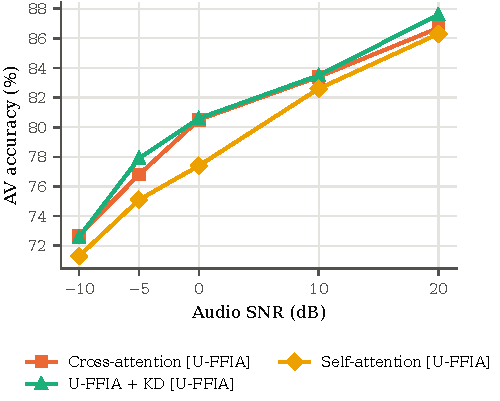
\includegraphics[width=\columnwidth]{figures/robustness_snr.pdf}}{\fbox{\parbox{0.9\columnwidth}{\centering run \texttt{scripts/make\_paper\_assets.py}}}}
  \caption{Audio-visual accuracy as the audio SNR decreases.}
  \label{fig:robust}
\end{figure}

\subsection{Evaluation protocol and data leakage}
\label{sec:protocols}
Table~\ref{tab:protocols} evaluates the same model under the three protocols of Sec.~\ref{sec:setup}:
\resOfficialAcc\,\% on the official split, \resKfoldAcc\,\% under 5-fold CV, and \resGroupedAcc\,\% on
the session-disjoint split.
\todo{If the session-disjoint accuracy is markedly lower, state that clip-level random splits
overestimate generalisation on AV-FFIA, and that published results above 95\% should be read with this
in mind.}

\begin{table}[t]
  \centering
  \caption{One model under three evaluation protocols.}
  \label{tab:protocols}
  \footnotesize
  \resizebox{\columnwidth}{!}{\begin{tabular}{lrrr}
\toprule
Evaluation protocol & Runs & Acc. & F1 \\
\midrule
Official code split (700/700 per class) & -- & -- & -- \\
5-fold stratified CV & -- & -- & -- \\
Session-disjoint (whole recording dates) & -- & -- & -- \\
\bottomrule
\end{tabular}
}
\end{table}

\subsection{Per-class analysis}
\label{sec:perclass}
Table~\ref{tab:perclass} and Fig.~\ref{fig:confusion} give the per-class F1 and the confusion matrix
of HyperAVNet-Q (KD).
\todo{Discuss the dominant confusions, expected between the adjacent intensities Weak and Medium,
and how much the audio stream contributes to separating them.}

\begin{table}[t]
  \centering
  \caption{Per-class F1 of HyperAVNet-Q (KD), official split.}
  \label{tab:perclass}
  \footnotesize
  \begin{tabular}{lr}
\toprule
Class & F1 (\%) \\
\midrule
None & -- \\
Strong & -- \\
Medium & -- \\
Weak & -- \\
\bottomrule
\end{tabular}

\end{table}

\begin{figure}[t]
  \centering
  \IfFileExists{figures/confusion.pdf}{\includegraphics[width=0.7\columnwidth]{figures/confusion.pdf}}{\fbox{\parbox{0.9\columnwidth}{\centering pending runs}}}
  \caption{Row-normalised confusion matrix (\%) of HyperAVNet-Q (KD), summed over seeds.}
  \label{fig:confusion}
\end{figure}

\subsection{Deployment}
\label{sec:deploy}
Table~\ref{tab:deploy} measures the cost of the two forms of the model on \resDeployDevice{} (batch 1).
In training form, every hypercomplex kernel is assembled from its $n$ blocks at each forward pass.
After reparameterisation (Sec.~\ref{sec:hyper}) the kernels are dense, and latency falls from
\resLatTrain\,ms to \resLatDeploy\,ms. The trade-off is explicit: the hypercomplex form stores and
transmits $n\times$ fewer parameters (2.14\,M), while the deployed dense form holds 7.88\,M parameters
in memory and runs faster. A device can therefore receive the compact model and expand it once at load
time.

\begin{table}[t]
  \centering
  \caption{Training-form versus reparameterised (deployed) model. Stored: parameters kept on disk and
  transmitted; Dense: parameters in memory after reparameterisation.}
  \label{tab:deploy}
  \footnotesize
  \IfFileExists{tables/deploy.tex}{\resizebox{\columnwidth}{!}{\begin{tabular}{lrrrrrr}
\toprule
Model & Stored (M) & Dense (M) & GMACs & Train-form (ms) & Deployed (ms) & Speed-up \\
\midrule
-- & -- & -- & -- & -- & -- & -- \\
\bottomrule
\end{tabular}
}}{\fbox{run \texttt{profile\_model.py --out}}}
\end{table}

\subsection{Limitations}
\label{sec:limitations}
Hypercomplex layers reduce stored parameters but not arithmetic, so the compute savings come from the
compact backbone design rather than from the algebra. AV-FFIA covers one species and one tank, and
generalisation to farm conditions (turbidity, foam, other species) remains to be shown. Finally, the
discrepancies in the public data release, and the variety of protocols in the literature, limit how
precisely results can be compared across papers.

%  Numbers come from tables/*.tex and tables/macros.tex, generated by
%  scripts/make_paper_assets.py from the run folders. Re-run it after new runs.
%  Sentences marked \todo{} state a claim that must be checked against the
%  final numbers (keep, reverse or delete).
% ============================================================================
\section{Results}
\label{sec:results}

\subsection{Comparison with the state of the art}
\label{sec:main}
Table~\ref{tab:main} lists the published results on AV-FFIA with their protocols, followed by our models
under the official split. The distilled quaternion model, HyperAVNet-Q (KD), reaches
\resOurAcc\,\% accuracy (macro-F1 \resOurFone\,\%) with \resOurParams\,M parameters and
\resOurGMACs\,GMACs per clip. That is 10.1$\times$ fewer parameters and 13.1$\times$ fewer MACs than
U-FFIA~\cite{cui2024uffia}, and 16.4$\times$ / 51.6$\times$ fewer than the cross-attention model.
\todo{Position against the strongest comparable result: DynaGate-AV reports 96.4--96.5\% on the same
official split rule, and HMMF-Net 96.77\% under 5-fold CV (Table~\ref{tab:protocols}). State whether
HyperAVNet exceeds, matches or trails them; LDMF and HMKD use filtered subsets and are not comparable.}
Fig.~\ref{fig:acc_compute} places all models on an accuracy--compute plane.
Its single-modality heads reach \resOurAccA\,\% (audio) and \resOurAccV\,\% (video), against the
best published single-modality models, Pre-CNN10 (85.9\%) and Pretrained-S3D (89.8\%)~\cite{cui2024uffia}.

\begin{table*}[t]
  \centering
  \caption{Comparison on AV-FFIA. Compute is in GMACs per 2\,s clip; U-FFIA's ``FLOPs'' are MACs.
  Published numbers are quoted with their own protocol and are not directly comparable across
  protocols. $^\dagger$Not verified against the full paper (taken from secondary sources). Our
  rows: official split, mean $\pm$ std over three seeds.}
  \label{tab:main}
  \small
  \resizebox{\textwidth}{!}{\begin{tabular}{llrrrrl}
\toprule
Method & Mod. & Params (M) & GMACs & Acc. (\%) & F1 (\%) & Protocol \\
\midrule
Pre-CNN10~\cite{cui2024uffia} & A & 5.00 & 3.347 & 85.9 & -- & paper split \\
Pretrained-S3D~\cite{cui2024uffia} & V & 7.90 & 22.826 & 89.8 & -- & paper split \\
Self-attention~\cite{cui2024uffia} & AV & 47.70 & 68.404 & 89.2 & -- & paper split \\
MBT~\cite{cui2024uffia} & AV & 47.69 & 68.690 & 72.4 & -- & paper split \\
Cross-attention~\cite{cui2024uffia} & AV & 35.08 & 60.933 & 91.7 & -- & paper split \\
U-FFIA + KD~\cite{cui2024uffia} & AV & 21.63 & 15.488 & 90.7 & -- & paper split \\
\midrule
ACAF-Net~\cite{acafnet2025}$^\dagger$ & AV & -- & -- & 95.4 & -- & random split \\
DynaGate-AV (Light)~\cite{dynagate2026} & AV & -- & 5.290 & 96.4 & -- & official split, 19,963 clips \\
HMMF-Net~\cite{hmmfnet2026}$^\dagger$ & AV & 3.99 & 1.002 & 96.8 & 96.9 & 5-fold CV \\
HMKD~\cite{hmkd2026}$^\dagger$ & AV & -- & -- & 97.5 & -- & 26,843-pair holdout \\
LDMF~\cite{ldmf2026}$^\dagger$ & AV & 7.10 & -- & 98.2 & -- & filtered subset \\
\midrule
Real late-concat baseline (ours, re-run) & AV & -- & -- & -- & -- & official split \\
Teacher: CNN10 + S3D + HCF & AV & -- & -- & -- & -- & official split \\
Teacher: EfficientAT + MoViNet-A0 + HCF & AV & -- & -- & -- & -- & official split \\
HyperAVNet-Q (no KD) & AV & -- & -- & -- & -- & official split \\
\textbf{HyperAVNet-Q (KD)} & AV & -- & -- & -- & -- & official split \\
HyperAVNet-P (pretrained, no KD) & AV & -- & -- & -- & -- & official split \\
HyperAVNet-P (pretrained, KD) & AV & -- & -- & -- & -- & official split \\
HyperAVNet-O (KD) & AV & -- & -- & -- & -- & official split \\
\bottomrule
\end{tabular}
}
\end{table*}

\begin{figure}[t]
  \centering
  \IfFileExists{figures/acc_vs_compute.pdf}{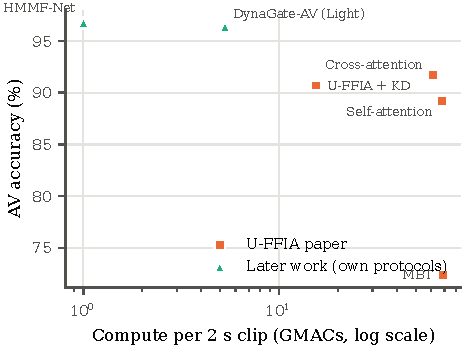
\includegraphics[width=\columnwidth]{figures/acc_vs_compute.pdf}}{\fbox{\parbox{0.9\columnwidth}{\centering run \texttt{scripts/make\_paper\_assets.py}}}}
  \caption{Accuracy versus compute (log scale) on AV-FFIA. Published models are plotted at their
  reported values and protocols; HyperAVNet uses the official split.}
  \label{fig:acc_compute}
\end{figure}

\subsection{Where to fuse: the deep-to-early study}
\label{sec:depth}
Table~\ref{tab:depth} and Fig.~\ref{fig:depth} vary the fusion set $\mathcal{S}$. Late fusion
($\mathcal{S}=\{3\}$) gives \resLateAcc\,\%; progressive fusion from stage~1 gives \resProgAcc\,\%;
the best setting is $\mathcal{S}=\resBestDepth$. Fusion is nearly free in compute: each additional HCF
stage costs about 0.17\,M parameters and under 0.02\,GMACs. Disabling the cross-modal feedback of
Eq.~\eqref{eq:feedback} at $\mathcal{S}=\{1,2,3\}$ gives \resNoFeedbackAcc\,\%.
\todo{Interpret: does accuracy grow as fusion moves earlier, saturate, or peak at mid-level stages
(an inverted U)? Does feedback help, and does the gain concentrate on Weak and Medium? Use the
single-stage rows to locate the most useful depth.}

\begin{table}[t]
  \centering
  \caption{Fusion depth (deep to early) and cross-modal feedback. Mean $\pm$ std, official split.}
  \label{tab:depth}
  \footnotesize
  \setlength{\tabcolsep}{3pt}
  \resizebox{\columnwidth}{!}{\begin{tabular}{lrrrrrr}
\toprule
Fusion stages $\mathcal{S}$ & Params (M) & GMACs & Acc. & F1 & A-only & V-only \\
\midrule
$\{3\}$ (late) & -- & -- & -- & -- & -- & -- \\
$\{2,3\}$ & -- & -- & -- & -- & -- & -- \\
$\{1,2,3\}$ & -- & -- & -- & -- & -- & -- \\
$\{0,1,2,3\}$ & -- & -- & -- & -- & -- & -- \\
\midrule
$\{0\}$ & -- & -- & -- & -- & -- & -- \\
$\{1\}$ & -- & -- & -- & -- & -- & -- \\
$\{2\}$ & -- & -- & -- & -- & -- & -- \\
\midrule
$\{1,2,3\}$ w/o feedback & -- & -- & -- & -- & -- & -- \\
\bottomrule
\end{tabular}
}
\end{table}

\begin{figure}[t]
  \centering
  \IfFileExists{figures/fusion_depth.pdf}{\includegraphics[width=\columnwidth]{figures/fusion_depth.pdf}}{\fbox{\parbox{0.9\columnwidth}{\centering pending runs \texttt{A\_fs*}}}}
  \caption{Accuracy as fusion moves from the last stage to all stages, with and without feedback.}
  \label{fig:depth}
\end{figure}

\subsection{Effect of the hypercomplex algebra}
\label{sec:algebra}
Table~\ref{tab:algebra} and Fig.~\ref{fig:algebra} replace every hypercomplex layer of the network with
algebra $\mathbb{A}_n$. All variants share the architecture and compute and differ only in weight
sharing. The real network ($n=1$, 7.88\,M parameters) reaches \resRealAcc\,\%, the quaternion network
(2.14\,M) \resQuatAcc\,\% and the octonion network (1.24\,M) \resOctAcc\,\%.
\todo{Interpret: if accuracy is maintained or improved down to $n=4$ or $n=8$, the Hamilton
weight sharing acts as a useful structural prior on a dataset of this size; report where accuracy
starts to drop.}

\begin{table}[t]
  \centering
  \caption{Algebra of the whole network. Compute is identical for all $n$.}
  \label{tab:algebra}
  \footnotesize
  \resizebox{\columnwidth}{!}{\begin{tabular}{lrrrr}
\toprule
Algebra & Params (M) & GMACs & Acc. & F1 \\
\midrule
Real ($n{=}1$) & -- & -- & -- & -- \\
Complex ($n{=}2$) & -- & -- & -- & -- \\
Quaternion ($n{=}4$) & -- & -- & -- & -- \\
Octonion ($n{=}8$) & -- & -- & -- & -- \\
Sedenion ($n{=}16$) & -- & -- & -- & -- \\
\bottomrule
\end{tabular}
}
\end{table}

\begin{figure}[t]
  \centering
  \IfFileExists{figures/algebra.pdf}{\includegraphics[width=\columnwidth]{figures/algebra.pdf}}{\fbox{\parbox{0.9\columnwidth}{\centering pending runs \texttt{B\_n*}}}}
  \caption{Accuracy against parameter count for real, complex, quaternion, octonion and sedenion networks.}
  \label{fig:algebra}
\end{figure}

\subsection{Fusion operator, regularisers and front-end}
\label{sec:operators}
Table~\ref{tab:ops} compares HCF with a hypercomplex attention bottleneck (MBT) at equal parameters,
and with gated concatenation. HCF with quaternion components gives \resHCFAcc\,\% and MBT
\resMBTAcc\,\%. In~\cite{cui2024uffia}, MBT also trailed cross-attention by a wide margin
(72.4\% vs.\ 91.7\%), which the authors attributed to attending to the modalities one after the other.
\todo{State whether parallel reading plus Hamilton mixing closes this gap, and whether octonion
components (four extra interaction terms, same parameters) help.}
The lower block of Table~\ref{tab:ops} isolates modality dropout, the auxiliary heads and the SimPF
front-end~\cite{liu2023simpf}.

\begin{table}[t]
  \centering
  \caption{Fusion operator (top), regularisers (middle) and audio front-end (bottom).}
  \label{tab:ops}
  \footnotesize
  \setlength{\tabcolsep}{3pt}
  \resizebox{\columnwidth}{!}{\begin{tabular}{lrrrrr}
\toprule
Variant & Params (M) & Acc. & F1 & A-only & V-only \\
\midrule
HCF, complex components & -- & -- & -- & -- & -- \\
HCF, quaternion components & -- & -- & -- & -- & -- \\
HCF, octonion components & -- & -- & -- & -- & -- \\
Hypercomplex MBT & -- & -- & -- & -- & -- \\
Gated concatenation & -- & -- & -- & -- & -- \\
\midrule
w/o modality dropout ($p{=}0$) & -- & -- & -- & -- & -- \\
modality dropout $p{=}0.25$ & -- & -- & -- & -- & -- \\
w/o auxiliary heads & -- & -- & -- & -- & -- \\
\midrule
SimPF front-end ($k{=}0.5$) & -- & -- & -- & -- & -- \\
\bottomrule
\end{tabular}
}
\end{table}

\subsection{Which teacher? Teacher ablation}
\label{sec:teachers}
Table~\ref{tab:teachers} reports each teacher's audio-visual and unimodal accuracy, and the accuracy
of the student distilled from it; $\Delta$ is student minus teacher. Fig.~\ref{fig:teachers} plots
student against teacher accuracy. Distillation from the default teacher (CNN10 + S3D,
\resTeacherAcc\,\%) changes the student's accuracy by \resKDGain\ points over the same student trained
without a teacher (\resNoKDAcc\,\%).
\todo{Interpret: does a stronger teacher yield a stronger student, or does the compact HMKD pair (T10,
about 1\,GMAC) distil as well as the larger teachers? Do the transformer teachers (T6, T8, T9) under-perform
on AV-FFIA, as AST and ViViT did in~\cite{cui2024uffia}?}

\begin{table*}[t]
  \centering
  \caption{Teacher ablation. Teacher params (M) and GMACs include the HCF fusion network. Student:
  HyperAVNet-Q distilled from that teacher. $\Delta$ = student $-$ teacher accuracy.}
  \label{tab:teachers}
  \small
  \resizebox{\textwidth}{!}{\begin{tabular}{llrrrrrrr}
\toprule
ID & Audio / video teacher & Params & GMACs & Teacher AV & A-only & V-only & Student & $\Delta$ \\
\midrule
T1 & CNN10 / S3D & -- & -- & -- & -- & -- & -- & -- \\
T2 & CNN14 / S3D & -- & -- & -- & -- & -- & -- & -- \\
T3 & CNN10 / R(2+1)D-18 & -- & -- & -- & -- & -- & -- & -- \\
T4 & CNN10 / ConvNeXt-T (frames) & -- & -- & -- & -- & -- & -- & -- \\
T5 & EffNet-B0 (mel) / S3D & -- & -- & -- & -- & -- & -- & -- \\
T6 & AST / VideoMAE-B & -- & -- & -- & -- & -- & -- & -- \\
T7 & CNN10 / X3D-M & -- & -- & -- & -- & -- & -- & -- \\
T8 & AST / S3D & -- & -- & -- & -- & -- & -- & -- \\
T9 & CNN10 / VideoMAE-B & -- & -- & -- & -- & -- & -- & -- \\
T10 & EfficientAT / MoViNet-A0 & -- & -- & -- & -- & -- & -- & -- \\
\midrule
-- & no teacher (no KD) & -- & -- & -- & -- & -- & -- & -- \\
\bottomrule
\end{tabular}
}
\end{table*}

\begin{figure}[t]
  \centering
  \IfFileExists{figures/teacher_student.pdf}{\includegraphics[width=\columnwidth]{figures/teacher_student.pdf}}{\fbox{\parbox{0.9\columnwidth}{\centering pending teacher runs}}}
  \caption{Teacher accuracy against the accuracy of the student distilled from it (dashed: no distillation).}
  \label{fig:teachers}
\end{figure}

\subsection{Robustness to noise and missing modalities}
\label{sec:robustness}
Table~\ref{tab:robust} and Fig.~\ref{fig:robust} follow the robustness protocol of~\cite{cui2024uffia}.
\todo{Compare the degradation at $-10$\,dB with U-FFIA (90.7\%$\to$72.6\%) and cross-attention
(91.7\%$\to$72.7\%), only if the same bubble and pump noise was used; otherwise describe the results
as indicative. Discuss the missing-modality columns: the auxiliary heads and masked training should
keep useful accuracy when one modality is absent.}

\begin{table*}[t]
  \centering
  \caption{Robustness. Audio noise at the given SNR (U-FFIA protocol); Dark: video intensities
  $\times0.25$; Noise: Gaussian video noise, $\sigma^{2}=0.2$; $-$A / $-$V: audio / video absent.
  Published rows from~\cite{cui2024uffia} (bubble and pump noise).}
  \label{tab:robust}
  \small
  \resizebox{\textwidth}{!}{\begin{tabular}{lrrrrrrrrrr}
\toprule
Method & Clean & -10\,dB & -5\,dB & +0\,dB & +10\,dB & +20\,dB & Dark & Noise & $-$A & $-$V \\
\midrule
Cross-attention~\cite{cui2024uffia} & 91.7 & 72.7 & 76.8 & 80.5 & 83.4 & 86.7 & -- & -- & -- & -- \\
U-FFIA + KD~\cite{cui2024uffia} & 90.7 & 72.6 & 77.9 & 80.6 & 83.5 & 87.6 & -- & -- & -- & -- \\
Self-attention~\cite{cui2024uffia} & 89.2 & 71.3 & 75.1 & 77.4 & 82.6 & 86.3 & -- & -- & -- & -- \\
\midrule
Teacher (CNN10 + S3D) & -- & -- & -- & -- & -- & -- & -- & -- & -- & -- \\
\textbf{HyperAVNet-Q (KD)} & -- & -- & -- & -- & -- & -- & -- & -- & -- & -- \\
\bottomrule
\end{tabular}
}
\end{table*}

\begin{figure}[t]
  \centering
  \IfFileExists{figures/robustness_snr.pdf}{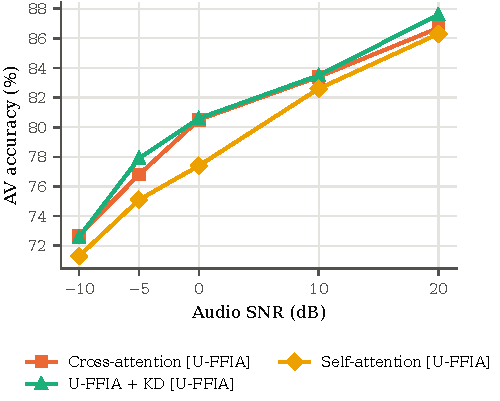
\includegraphics[width=\columnwidth]{figures/robustness_snr.pdf}}{\fbox{\parbox{0.9\columnwidth}{\centering run \texttt{scripts/make\_paper\_assets.py}}}}
  \caption{Audio-visual accuracy as the audio SNR decreases.}
  \label{fig:robust}
\end{figure}

\subsection{Evaluation protocol and data leakage}
\label{sec:protocols}
Table~\ref{tab:protocols} evaluates the same model under the three protocols of Sec.~\ref{sec:setup}:
\resOfficialAcc\,\% on the official split, \resKfoldAcc\,\% under 5-fold CV, and \resGroupedAcc\,\% on
the session-disjoint split.
\todo{If the session-disjoint accuracy is markedly lower, state that clip-level random splits
overestimate generalisation on AV-FFIA, and that published results above 95\% should be read with this
in mind.}

\begin{table}[t]
  \centering
  \caption{One model under three evaluation protocols.}
  \label{tab:protocols}
  \footnotesize
  \resizebox{\columnwidth}{!}{\begin{tabular}{lrrr}
\toprule
Evaluation protocol & Runs & Acc. & F1 \\
\midrule
Official code split (700/700 per class) & -- & -- & -- \\
5-fold stratified CV & -- & -- & -- \\
Session-disjoint (whole recording dates) & -- & -- & -- \\
\bottomrule
\end{tabular}
}
\end{table}

\subsection{Per-class analysis}
\label{sec:perclass}
Table~\ref{tab:perclass} and Fig.~\ref{fig:confusion} give the per-class F1 and the confusion matrix
of HyperAVNet-Q (KD).
\todo{Discuss the dominant confusions, expected between the adjacent intensities Weak and Medium,
and how much the audio stream contributes to separating them.}

\begin{table}[t]
  \centering
  \caption{Per-class F1 of HyperAVNet-Q (KD), official split.}
  \label{tab:perclass}
  \footnotesize
  \begin{tabular}{lr}
\toprule
Class & F1 (\%) \\
\midrule
None & -- \\
Strong & -- \\
Medium & -- \\
Weak & -- \\
\bottomrule
\end{tabular}

\end{table}

\begin{figure}[t]
  \centering
  \IfFileExists{figures/confusion.pdf}{\includegraphics[width=0.7\columnwidth]{figures/confusion.pdf}}{\fbox{\parbox{0.9\columnwidth}{\centering pending runs}}}
  \caption{Row-normalised confusion matrix (\%) of HyperAVNet-Q (KD), summed over seeds.}
  \label{fig:confusion}
\end{figure}

\subsection{Deployment}
\label{sec:deploy}
Table~\ref{tab:deploy} measures the cost of the two forms of the model on \resDeployDevice{} (batch 1).
In training form, every hypercomplex kernel is assembled from its $n$ blocks at each forward pass.
After reparameterisation (Sec.~\ref{sec:hyper}) the kernels are dense, and latency falls from
\resLatTrain\,ms to \resLatDeploy\,ms. The trade-off is explicit: the hypercomplex form stores and
transmits $n\times$ fewer parameters (2.14\,M), while the deployed dense form holds 7.88\,M parameters
in memory and runs faster. A device can therefore receive the compact model and expand it once at load
time.

\begin{table}[t]
  \centering
  \caption{Training-form versus reparameterised (deployed) model. Stored: parameters kept on disk and
  transmitted; Dense: parameters in memory after reparameterisation.}
  \label{tab:deploy}
  \footnotesize
  \IfFileExists{tables/deploy.tex}{\resizebox{\columnwidth}{!}{\begin{tabular}{lrrrrrr}
\toprule
Model & Stored (M) & Dense (M) & GMACs & Train-form (ms) & Deployed (ms) & Speed-up \\
\midrule
-- & -- & -- & -- & -- & -- & -- \\
\bottomrule
\end{tabular}
}}{\fbox{run \texttt{profile\_model.py --out}}}
\end{table}

\subsection{Limitations}
\label{sec:limitations}
Hypercomplex layers reduce stored parameters but not arithmetic, so the compute savings come from the
compact backbone design rather than from the algebra. AV-FFIA covers one species and one tank, and
generalisation to farm conditions (turbidity, foam, other species) remains to be shown. Finally, the
discrepancies in the public data release, and the variety of protocols in the literature, limit how
precisely results can be compared across papers.
